\documentclass[tcc]{ic}

\hypersetup{
    colorlinks = {true},
    linktocpage = {false},
    plainpages = {false},
    linkcolor = {Blue},
    citecolor = {Blue},
    urlcolor = {Red},
    unicode = {true},
    pdftitle = {Rapport des enseignements à l'IUT du 11-03-2024 au 12-04-2024}, 
    pdfauthor = {Alexis Déhu},
    pdfsubject = {Rapport de mes enseignements reçus à l'IUT de Mont-de-Marsan pour la quatrième période de ma deuxième année du 11-03-2024 au 12-04-2024},
    pdfkeywords = {enseignements, apprentissage, alternance, iut, but, rt, uppa, pau, mont, de, marsan, mont-de-marsan}
}

\usepackage{algorithm}
\usepackage{algpseudocode}
\usepackage[graphicx]{realboxes}

\makeatletter
\renewcommand{\ALG@name}{Algoritmo}
\renewcommand{\listalgorithmname}{List of \ALG@name s}
\makeatother

\newcolumntype{Y}{>{\centering\arraybackslash}X}

\begin{document}

    % Inclui o preâmbulo do documento (Informações da capa e contracapa)
    \titulo{Rapport des enseignements à l’IUT}

\autor{Alexis Déhu}{a.dehu@aditu.fr}{}


\orientador{M. Angel Abénia}{abenia@univ-pau.fr}{}{}{}
%\examinador{Mr. Guillaume Devesa}{g.devesa@aditu.fr}{}{}{}

\dataMesAno{Septembre}{2023}{}

    \selectlanguage{english}
    
    
    % Capa, contracapa e avaliadores
    \capa
    
    % \aprovacao
    
    % Agradecimentos
    % \begin{agradecimentos}

Obrigado

\end{agradecimentos}
    
    % Resumo e Abstract
    \begin{resumo}

    Cette deuxième période la plus longue d'enseignements à l'IUT (5 semaines) nous a permis d'aborder un vaste champ de compétences extrêmement utiles et intéressantes selon moi.
    \\ \\
    Nous avons couvert trois modules de notre parcours cybersécurité orienté vers la sécurisation du service DNS avec DNSsec, de la compréhension des attaques utilisées sur des protocoles répandus dans les réseaux locaux d'entreprises et de la compréhension des technologies et pratiques de chiffrement de nos données.
    \\
    Nous avons aussi aussi à manipuler et intégrer des pare-feux physiques dans un réseau local d'entreprise selon leur besoins.
    \\ \\
    Aspect télécommunications, nous avons abordés les réseaux cellulaires 2G, 3G, 4G et d'autres en profondeur, en parallèle avec l'étude physique et mathématique de moyens transmissions modernes d'émission-réception.
    \\ \\
    Un module intéressant était aussi consacré à l'automatisation de nos tâches d'administrations des systèmes et des réseaux. En complément de l'apprentissage d'un anglais professionnalisé et d'un travail sur notre communication.
    
    \palavrasChave{sécurisation; protocoles; ARP; ICMP; DNS; chiffrement; cryptographie; clés; chiffrement symétrique; chiffrement asymétrique; intégrité des données; confidentialité; authentification; authenticité; signature; certificat; fonctions mathématiques et algorithmiques; OFDM; COFDM; MIMO; CDMA; TDMA; FHSS; féseaux cellulaire; filtres numériques; filtres analogiques}
\end{resumo}
    %% \begin{abstract}
%     Lorem ipsum dolor sit amet, consectetur adipiscing elit. Duis elit tellus, vehicula in justo eget, fermentum aliquet nisi. In id quam mauris. Sed id vehicula libero. Quisque id tortor placerat, consequat ex sed, placerat ante. Ut dui nunc, placerat volutpat ipsum sit amet, dictum pellentesque lacus. Donec leo sem, dictum quis lacus at, ultricies sagittis elit. Mauris sit amet tortor efficitur, luctus justo sit amet, tincidunt tellus. Donec vulputate non risus at tincidunt. Sed accumsan at erat in aliquet. Sed consequat gravida bibendum. Sed fermentum metus sed ex lacinia mattis. Phasellus vel enim nisl. Proin tortor dui, luctus in erat a, dapibus convallis turpis. Maecenas vitae vulputate neque.

%     Etiam ac ante a lorem consectetur varius. Donec vitae dui porttitor, efficitur ante sed, aliquet lectus. Etiam aliquet mattis sagittis. Integer accumsan, est nec vehicula suscipit, nibh nisl varius ante, at convallis urna est dapibus massa. Orci varius natoque penatibus et magnis dis parturient montes, nascetur ridiculus mus. Praesent tempus dolor sit amet metus eleifend porta. Vestibulum eget viverra nulla. Mauris ac condimentum augue, quis molestie tortor. Duis ac condimentum tortor, sed ullamcorper nunc. Vivamus et suscipit arcu. Duis eget rutrum est, sed pellentesque leo. Nulla lorem lacus, faucibus vitae lectus eu, porttitor efficitur ante. Sed risus tortor, venenatis quis convallis non, blandit in orci. Morbi et neque hendrerit, consectetur magna vitae, consectetur dolor. Nam nec iaculis urna, vitae tincidunt eros. Ut pretium neque convallis turpis rutrum, nec dapibus est faucibus.
    
%     Quisque id laoreet ligula. In hac habitasse platea dictumst. Fusce scelerisque, nunc non lacinia maximus, lorem metus rutrum lacus, ac maximus dolor tellus at velit. Sed diam leo, interdum ut sapien at, finibus aliquam diam. Praesent vel erat id enim scelerisque fringilla. Aliquam cursus risus vulputate ex interdum, sit amet pretium augue semper. Curabitur eget risus eget nulla placerat ornare. Nam quis ornare ipsum. Duis id feugiat lectus. Phasellus vehicula leo id consequat porta. Aliquam ut massa malesuada, ultricies ipsum nec, euismod eros. In lacinia aliquet leo non mattis. Etiam semper neque risus, a condimentum diam euismod eget. Suspendisse vulputate viverra mauris, ac sollicitudin tellus placerat non. Nullam felis metus, congue sed neque ac, iaculis sollicitudin nisl.
    
%     \keywords{graphics processing; medical images; computer vision; deep learning; data augmentation;}
% \end{abstract}
    
    % Sumário
    \renewcommand*\contentsname{Table des matières}
    \tableofcontents
    \thispagestyle{empty}
    
    % Início dos capítulos
    \inicio
    \renewcommand{\figurename}{}
\mychapter{R4Cyber.09 Sécurité des Réseaux LAN (16h30)}{cap:r4c09} 
\lhead{R4Cyber.09 Sécurité des Réseaux LAN (16h30)}

\vspace*{0.2cm}%
      \large
      \href{}{\color{black}Enseignant\\M. Laurent Gallon}\\%
      \normalsize
\vspace*{0.5cm}%

Ce module portait sur la sécurisation des réseaux locaux d'entreprise. Dans celui-ci, nous avons revu le fonctionnement de protocoles réseaux utilisés dans les réseaux locaux d'entreprise, pour ensuite en voir une application utilisée pour des attaques courantes les utilisant.
\\ \\
Pour se prémunir de ces attaques et mieux les comprendre, nous les avons expérimentées dans des environnements contrôlés, puis nous avons mis en place des mécanismes de protection pour s'en prémunir.

\section{Forger des paquets volontairement malicieux sur un réseau}

% forger ses paquets avec scapy

Pour simuler les attaques, nous avons appris à initier un comportement anormal sur un réseau en modifiant les informations que l'on envoie sur celui-ci.
\\ \\
Notre intention dans une attaque est de générer un comportement anormal sur une machine ciblée. Pour ce faire, nous devions forger des demandes malicieuses pour provoquer une réaction attendue chez elle.
\\ \\
Nous avons donc appris à utiliser l'outil \texttt{Scapy} pour générer tout type de trafic réseau, en modifiant à souhait la composition de nos demandes. Nous pouvions notamment à l'issue usurper l'identité d'un hôte sur le réseau pour que celui-ci reçoive des communications que nous avions initiées à sa place.

\section{Prise en main des attaques courantes}

Suite à cet apprentissage, nous avons pu commencer notre étude des attaques étudiées théoriquement. Nous en avons notamment montées deux : l'attaque de l'homme du milieu par empoisonnement de la table ARP, et l'attaque du déni de service par rebond. Je vais en présenter une ici.

\subsection{Attaque de l'homme du milieu par empoisonnement ARP}

% mitm par arp poisoning

Pour la première, il nous fallait revoir le fonctionnement du protocole ARP. Celui-ci est indispensable pour utiliser le protocole IPv4, servant à trouver qui possède une adresse IP dans un réseau local.
\\ \\
Notre objectif, côté attaquant, fut de dire dans un réseau local à toutes les machines que nous étions maintenant leur passerelle, ou leur "box". Nous disions à haute voix notre nouvel emplacement pour usurper identité de la vraie passerelle, afin que les machines pensent que si elles veulent accéder à Internet, qu'elles le fassent par nous.
\\ \\
Nous avions par la suite qu'à renvoyer les demandes de connexion vers la vrai passerelle, et renvoyer les réponses aux victimes. Nous pouvions donc voir les connexions que les machines effectuées sur Internet, et si non protégées : voir leur contenu.

\begin{figure}[H]
    \centering
    \captionsetup{justification=centering}
    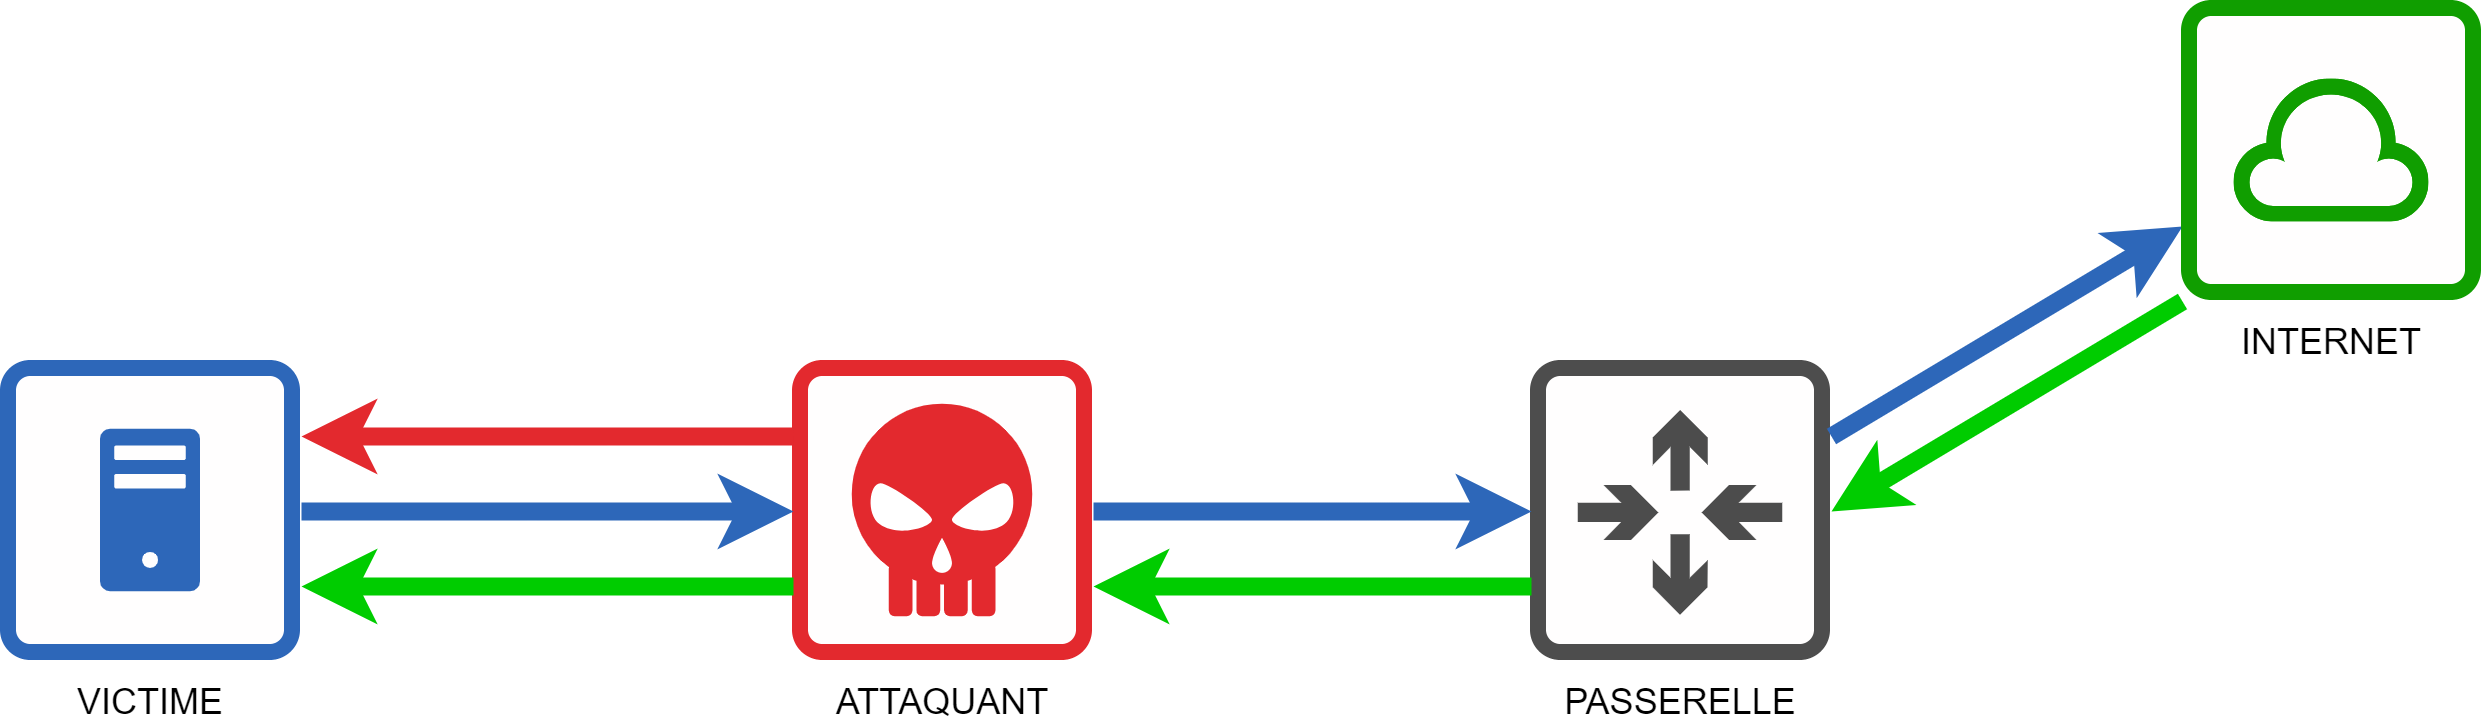
\includegraphics[width=\textwidth - \textwidth / 20]{ressources/arp_poisoning_2.png}
    \figurename
    \caption{Illustration de l'attaque par l'homme du milieu par empoisonnement de table ARP. L'attaquant informe qu'il est le nouvel emplacement de la passerelle du réseau pour intercepter les requêtes et les réponses attendues pour la victime.}
    \label{fig:poste}
\end{figure}

% icmp smurf (ip source = victime, ip dest. = broadcast)

    \renewcommand{\figurename}{}
\mychapter{R4Cyber.10 Cryptographie (10h30)}{cap:r4c10} 
\lhead{R4Cyber.10 Cryptographie (10h30)}

\vspace*{0.2cm}%
      \large
      \href{}{\color{black}Enseignant\\M. Laurent Gallon}\\%
      \normalsize
\vspace*{0.5cm}%

% algorithmes de cryptographie
% fonctions de hashage
% chaîne PKI

Ce module nous a plongé dans la compréhension des fondamentaux de la cryptographie, à l'intérieur du chiffrement de nos données. Nous y avons abordé les principes d'authenticité, de confidentialité et d'intégrité des informations transférées lors d'un échange.
\\ \\
La cryptologie a été abordée via une approche scientifique et mathématiques théoriques dans un premier temps, puis par une approche pratique avec une application dans un système de messagerie et de connexion à des machines distantes sécurisée.

\section{Enseignements théoriques}

% algorithmes de cryptographie
% fonctions de hashage
% chaîne PKI

% rsa
% dh

Lors des travaux pratiques et des cours magistraux, nous avons vu les schémas de fonctionnement des algorithmes courants de cryptographie, des fonctions de hachage et de la chaîne PKI.
\\ \\
Nous avons étudié les protocoles RSA et Diffie-Hellman pour nous intéresser à la cryptographie.  Le premier de la famille des clés symétriques et le deuxième des asymétriques, leur objectif commun est de former un couple de clés (distrinctes pour l'asymétrique, identiques pour la symétrique) que seuls les communiquant connaîtront et utiliseront pour s'échanger des informations.
\\ \\
Problème de la clé symétrique : on ne peut pas distinguer l'une personne de l'autre utilisant la clé. Ainsi, la paire de clés asymétriques permet une authentification de l'expéditeur du message, utilisant sa clé unique privée pour chiffre son message que le ou les réceptionneurs pourront déchiffrer s'ils ont en leur possession une clé dite "publique" que tout le monde pourra utiliser pour ouvrir le message chiffré.
\\ \\
Le système de chiffrement asymétrique est notamment utilisant lors de vos navigations WEB pour être certain de l'identité de \texttt{google.com} par exemple : tout le monde est en possession de la clé publique sur leur navigateur mais uniquement \texttt{google}, qui lui seul possède sa clé privée, pourra initier un échange chiffré (et non un autre site usurpateur).

\subsection{Application dans le monde réel}

Nous avons appliqué les concepts dans le cadre de chiffrement de courriels entre deux adresses. En effet, toujours en suivant le principe des clés asymétriques : nous avons vérifié l'authenticité de l'expéditeur, l'authenticité du message mais aussi son intégrité en vérifiant son empreinte.
\\ \\
La vérification de l'empreinte permet de vérifier si le message a été modifié en cours de route. Cependant, celui-ci ne doit pas être modifié lui aussi... C'est pour cela que lui aussi est chiffré avec le message pour que le destinataire en déchiffrant le message puisse le comparer à son empreinte et être certain de son intégrité.

% messagerie sécurisée
% connexion à des machines à distance
    \renewcommand{\figurename}{}
\mychapter{R4Cyber.11 Sécurisation des services réseaux (16h30)}{cap:r4c11} 
\lhead{R4Cyber.11 Sécurisation des services réseaux (16h30)}

\vspace*{0.2cm}%
      \large
      \href{}{\color{black}Enseignant\\M. Jean-Jacques Bascou}\\%
      \normalsize
\vspace*{0.5cm}%

% dnssec

Nous avons étudié pour le module R4Cyber.11 des principes de sécurisation d'un protocole constamment utilisé mais protégé que tardivement : le protocole DNS.
\\ \\
Le protocole DNS sert à effectuer des résolutions de noms sur Internet. Pour donner un exemple, vous retenez le nom symbolique \texttt{youtube.com} pour accéder aux serveur de YouTube; et non pas les adresses IP des serveurs sur Internet. Les serveurs DNS servent à faire correspondre des noms symboliques à des adresses IP tangibles par vos machines.
\\ \\
Les noms symboliques fonctionnent par arborescence. Pour `www.univ-pau.fr`, en premier sera demandé le serveur DNS gérant \texttt{.fr} pour lui demander l'emplacement de \texttt{univ-pau} (l'adresse IP du serveur DNS gérant cette zone de sites), qui lui saura nous dire pour quelle adresse IP il possède un enregistrement pour \texttt{www}.
\\ \\
Ainsi, si les serveurs dirigeants vers les \texttt{.fr}, les \texttt{.com} etc. tomberaient en panne : plus personne ne saurait savoir où sont les sites sur Internet (à moins de déjà connaître leurs adresses). Pour ce faire, sont utilisés et connus 13 serveurs DNS dit racines, gérés par les plus grandes sociétés pour que la résolution des noms puissent toujours opérer sur Internet. Nous faisons confiance à la sécurité de ces 13 serveurs, leur disponibilité et leur véracité : mais quand est-il si l'on doit le faire pour nous ?
\\ \\
Ainsi, nous avons pu commencer à gérer notre zone DNS (par exemple \texttt{adehu.univ-pau.fr}) et la sécuriser avec DNSSEC; qui est une suite de bonnes pratiques pour sécuriser son installation DNS.
\\ \\
Ainsi, nous avons vu comment authentifier nos serveurs DNS entre eux pour éviter qu'une personne mal intentionnée puisse se faire passer pour un serveur DNS voulant redistribuer nos informations. Signer nos zones gérées en utilisant une information donnée par le serveur DNS supérieur (dans notre exemple du \texttt{adehu.univ-pau.fr}, j'utilise une information de \texttt{univ-pau} pour lui dire que je gère bien (et moi seul) \texttt{adehu.}.
    \renewcommand{\figurename}{}
\mychapter{R4.01 Infrastructures de sécurité (7h30)}{cap:r401} 
\lhead{R4.01 Infrastructures de sécurité (7h30)}

\vspace*{0.2cm}%
      \large
      \href{}{\color{black}Enseignant\\M. Laurent Gallon}\\%
      \normalsize
\vspace*{0.5cm}%

Présent dans le tronc commun mais faisant appel aux notions de notre parcours Cybersécurité, le module Infrastructures de sécurité nous a plongé dans le fonctionnement des chiffrements de nos données et à la découverte des équipements et des principes de sécurité permettant la sécurisation de nos transmissions et des infrastrctures.
\\ \\
Ainsi, nous avons abordés l'ensemble des informations permettant la compréhension des mécanismes de filtrage et de contrôle des accès d'un réseau, les bases de la cryptographie, ainsi que les services, applications et infrastructures pour la sécurité.

\section{Enseignement et manipulation de pare-feux}

Nous avons pu voir en détail les métholodologies d'approche des règles d'un pare-feux, à mémoire d'états ou non. Un pare-feu se définit comme un équipement régissant les flux d'accès dans un réseau : telle personne a le droit d'accéder à cette ressource, celle-ci ne doit pas y accéder ou n'a pas besoin de cet accès...
\\ \\
Un pare-feu matériel n'est pas à confondre avec un pare-feu logiciel comme présent sur vos ordinateurs; ceux-ci régissent les activités des programmes installés sur vos machines, un équipement pare-feu régit l'activité d'un réseau pour gérer les flux et les accès.
\\ \\
Dans cette vision, nous avons élaboré des stratégies de sécurisation d'entreprises à moyenne et grande échelle. Nous y avons vu la réflexion derrière la confection d'un tableau de gestion d'accès, et son implémentation sur une machine pare-feu GNU/Linux.
\\ \\
Plusieurs notions avancées ont été couvert comme les DMZ \textit{zones démilitarisées} pour laisser une activité extérieure accéder à certaines ressources en dehors du réseau d'entreprise (dans le cas d'un hébergement dans les locaux d'un site WEB, d'une application métier...). Nous avons aussi couvert le NAT \textit{translatation d'adresses}, les ACL \textit{règles d'accès} et les firewall-proxy pour restreindre les applications dans leur fonctionnement sur le réseau.
\\ \\
Nous avons ainsi mis en place lors de travaux pratiques une connexion multi-site via un réseau d'opérateur avec un accès distant sécurisé, des services réseaux avancées; tout cela en mettant en place une politique de sécurisation et de contrôles d'accès via des firewall-proxy.
    \renewcommand{\figurename}{}
\mychapter{R4.02 Transmissions avancées (24h)}{cap:r402} 
\lhead{R4.02 Transmissions avancées (24h)}

\vspace*{0.2cm}%
      \large
      \href{}{\color{black}Enseignant\\M. Christophe Baillot}\\%
      \normalsize
\vspace*{0.5cm}%

% pour sûr
% Les émetteurs-récepteurs de systèmes modernes (filtres numériques)
%% modulation IQ, application physique et mathématique
% Gestion des chemins multiples dans les airs
%% sauts de fréquences 2G



% metteur récépteur antennes
% mimo
% ofdm
% super hétérodyne,, 0IF
% cdma

Module d'enseignement portant sur la physique des télécommunications, nous y avons abordé les prémices des notions relatives à la transmission sur antennes pour de la radiophonie, de la téléphonie et des données (Wi-Fi...).
\\ \\
Pour cela, nous avons revu les systèmes d'émission et réception sur des systèmes modernes par les filtres numériques; et plus particulièrement en abordant dans les domaines mathématique et physique le fonctionnement de la modulation IQ.
\\ \\
Par la suite, nous avons commencé à voir les problématiques liées à l'utilisation de l'espace comme support de transmission. Nous y avons premièrement abordé la problématique des chemins multiples d'une onde dans un milieu urbain, ainsi que les technologies qui ont permis de s'en prémunir.
\\ \\
La suite de ce module fut celui R4.03, où nous continuions notre avancée prise par l'apprentissage sur ce module.

\section{Les émetteurs-récepteurs de systèmes modernes (filtres numériques)}

Pour revoir les émissions et les réceptions théoriquement, nous avons abordé de manière poussée la modulation IQ. En effet, la modulation permet à une suite d'information d'être modifiée pour mieux circuler sur son support (ici, l'air).
\\ \\
La modulation IQ elle se sert de la phase d'un signal pour définir ses états significatifs (0, 1; ou 00, 01, 11...) que l'on devra discerner à la réception pour interpréter le signal, et retrouver les informations.
\\ \\
Dans cette optique, nous avons d'abord étudié physiquement le schéma comportemental de l'émission sur modulateur IQ, en représentant dans l'espace des fréquences et du temps le signal à différents endroit du dispositif.
\\ \\
Nous avons par la suite caractérisé mathématiquement la raison du comportement du signal à ces emplacements, suite de multiplication par des sinusoïdes à l'envoi et la réception.
\\ \\
En conséquent, nous avons étudié en profondeur le fonctionnement et la mathématique d'un système de transmission en télécoms, la modulation IQ. Extrêmement enrichissant et contingent à la compréhension des composant d'un système (filtres, amplificateurs, mélangeurs, oscillateurs locaux...).

\section{Gestion des problématique des télécoms dans les airs}

Chaque support de transmission a ses avantages et ses inconvénients, l'air ne faisant exception. Nous avons commencé à aborder une des problématiques majeures que procure l'air à son utilisation : une onde se propage librement dans l'air, si relief urbain celle-ci peut rebondir sur les bâtiments et revenir à la réception plusieurs fois dû au temps des différents trajets qu'elle aura emprunté.
\\ \\
Le problème des trajets multiples a été contré dès la 2G avec les sauts de fréquences (FHSS, 1 message une fréquence et on tourne), avec de l'étalement de spectre CDMA pour la 3G et l'OFDM avec son attente pour la 4G.
\\ \\
Nous avons étudié ces trois technologies, leurs fonctionnement évolutions et avantages au fil du temps, sur le plans physiques notamment. Nous avons aussi entrevu la CDMA utilisé sur du Wi-Fi, Wimax et 5G.


% En effet, nous avons premièrement étudié les notions d'émetteurs-récepteurs superhétérodyne et 0 IF. Nous y avons vu la composition des émetteurs et des récepteurs dit superhétérodynes, mélangeant le sinus et le cosinus d'un signal pour l'émetteur et les transposer sur une même fréquence intermédiaire, pour la récupérer côté récepteur et dissocier le signal sinus et cosinus en remélangant par les mêmes fréquences.
% \\ \\
% Pour le récépteur sans fréquence image (0 IF), le principe est de sous échantilloner de telle sorte que les deux fréquences réçues se retrouve à s'amplifier en 0 Hz.
% \\ \\
% Nous avons aussi abordé le multiplexage fréquentiel avec le CDMA \textit{accès multiple par répartition en code }. Nous avons aussi abordé l'OFDM utilisé en 4G; permettant de chevaucher des fréquences dans un spectre (à interval extrêmement précis) sans que celles-ci ne se perturbent : ce qui permet d'envoyer la même quantité d'informations dans une largeur spectrale réduite.
% \\ \\
% Nous avons aussi étudié la technologie MIMO en s'appuyant sur les avantages d'utiliser de la diversité d'antennes (pour mieux recevoir un signal en se servant du nombre d'antennes pour diminuer le rapport signal sur bruit) ou du multiplexage spatial (utiliser plusieurs antennes pour envoyer plusieurs informations, qu'on doit pouvoir décorreler entre chacune d'entre elles).
    \renewcommand{\figurename}{}
\mychapter{R4.03 Physique des télécoms (27h)}{cap:r403} 
\lhead{R4.03 Physique des télécoms (27h)}

\vspace*{0.2cm}%
      \large
      \href{}{\color{black}Enseignant\\M. Christophe Baillot}\\%
      \normalsize
\vspace*{0.5cm}%

Pour ce deuxième module exclusif à la physique des télécoms, nous avons abordés des notions avancées en électronique touchant globalement aux réseaux cellulaires dans les télécoms, faisant sens à notre module R4.04 et R4.02.
\\ \\
Nous y avons vu les émetteurs et récepteurs superhétérodynes et 0 IF, de la modulation multi-porteuse OFDM

\section{Les systèmes de transmission étudiés}

Nous avons étudié les systèmes de transmission superhétérodynes, en soit des systèmes de transmission modulant deux fois le signal sur une fréquence porteuse et sur une fréquence intermédiaire, cette dernière pour le transport.
\\ \\
Leur intérêt est de pouvoir recentrer le signal sur une fréquence particulière tout en conservant la modulation permise par la fréquence porteuse. À la réception, remultiplier le signal reçu par la même fréquence intermédiaire permettra avec un filtre de récupérer le signal transporté avec transposition.
\\ \\
Le récepteur 0 IF, pour aucune fréquence intermédiaire (ou image), permet de récupérer le signal modulé en bande de base en échantillonnant de telle sorte que le repliement de spectre permette que le signal reçu s'amplifie en \texttt{0 Hz}.
\\ \\
Ce dernier est utilisant à très hautes fréquences, les systèmes actuels ne pouvant échantillonner des valeurs arrivant aussi rapidement (à hautes fréquences).

Ainsi, nous avons vu successivement plusieurs technologies, chacune répondant petit à petit à des problématiques grace aux avancées faites

\subsection{Compréhension des principes liés au MIMO}

Nous avons finalement abordé les technologies MIMO et MISO, utilisant des émetteurs à plusieurs antennes, et/ou non des récepteurs à plusieurs antennes aussi.
\\ \\
Leur utilisation permette de mieux recevoir le signal, et d'en diminuer le rapport que l'on en voit avec le bruit. Ou d'envoyer une information d'antenne à antenne quand le nombre est réciproque des deux côtés (en décorélant les flux, envoyer X fois plus d'informations où X le nombre d'antennes).
    \renewcommand{\figurename}{}
\mychapter{R4.04 Réseaux cellulaires (27h)}{cap:r404} 
\lhead{R4.04 Réseaux cellulaires (27h)}

\vspace*{0.2cm}%
      \large
      \href{}{\color{black}Enseignant\\M. Yannick Lespine   }\\%
      \normalsize
\vspace*{0.5cm}%

Grand module dans les télécommunications, celui-ci nous a énormément appris sur les réseaux cellulaires notamment pour la téléphonie mobile. Reprenant des enseignements sur les antennes et la physique permettant le transport d'informations, le module R4.04 nous a plongé dans la compréhension des réseaux mobiles 2G, 3G et 4G; avec des parties applicables au Wi-Fi.
\\ \\
Est entendu réseau cellulaire un réseau couvrant une surface, découpé en petites zones alors dites cellules pour couvrir l'ensemble de la surface.
\\ \\
Ce principe est utilisé dans la téléphonie mobile (3G, 4G...). Ainsi, vous avez des antennes partout en France permettant de couvrir globalement le territoire. Les antennes couvrent une cellule.
\\\\
Appliqué à ceci, nous avons vu l'intérêt des pylônes pour les opérateurs et pourquoi sont-ils si haut. Nous avons aussi vu les ondes et fréquences délimitant les normes (GSM, 3G, 4G...), les technologies que celles-ci utilisent et ce très en profondeur.
\\ \\
Ainsi, nous avons vu en détails toutes les procédures de communication entre un appareil mobile, un pylône et le réseau, pour transférer de la données ou de la voix et les problèmes que cela engendre sur de grandes distances (chemins multiples). Nous avons notamment étudié comment un téléphone se raccorde à une antenne, comment le faire sonner, que ce passe-t-il lorsqu'il est en déplacement (voiture ou autre) et que l'on est en communication.
\\ \\
En travaux pratique, à l'aide d'analyseur de spectres : nous avons étudiés les signaux reçus des antennes aux alentours et comparé nos résultats avec nos connaissances. Nous avons aussi étudié la couverture réseau entre les villes de Mont-de-Marsan et Dax, les intérêts des opérateurs selon tels pylônes, couvertures...
    \renewcommand{\figurename}{}
\mychapter{R4.05 Automatisation des tâches d'administration (18h)}{cap:r405} 
\lhead{R4.05 Automatisation des tâches d'administration (18h)}

\vspace*{0.2cm}%
      \large
      \href{}{\color{black}Enseignant\\M. Philippe Arnould}\\%
      \normalsize
\vspace*{0.5cm}%

% préciser que repris prochaine période
    \renewcommand{\figurename}{}
\mychapter{R4.06 Anglais professionnel (15h)}{cap:r406} 
\lhead{R4.06 Anglais professionnel (15h)}

\vspace*{0.2cm}%
      \large
      \href{}{\color{black}Enseignant\\Jeff}\\%
      \normalsize
\vspace*{0.5cm}%

Reprenant les pas du module R3.11, Jeff a repris ses exercices de grammaires et les évaluations orales pour au mieux nous préparer à de futurs entretiens ou examens.
\\ \\
Les exactes mêmes principes ont été suivis : nous étudions des séries de plus en plus de notions en grammaire anglaise que nous devions savoir retenir et retranscrire à l'examen.
\\ \\
Mais aussi, savoir préparer et soutenir un oral entièrement en anglais, assuré sa grammaire dans celui-ci et répondre aux questions de la classe par la suite.
    \renewcommand{\figurename}{}
\mychapter{R4.07 Expression Communication 4 (15h)}{cap:r406} 
\lhead{R4.07 Expression Communication 4 (15h)}

\vspace*{0.2cm}%
      \large
      \href{}{\color{black}Enseignant\\M. Walter Rohrig}\\
      \normalsize
\vspace*{0.5cm}%

% contrôle théorique sur les enseignements
% mise en situation de résolution d'un prolblème

Ayant pour objectif d'améliorer notre communication en entreprise, ce module s'est vu être enrichissant en connaissances théoriques et pratiques pour communiquer plus efficacement. Pour ce faire, nous avons été évalués de manière théorique sur notre compréhension des notions abordées pour au mieux mener une conversation juste avec intérêt, et en pratique sur un atelier de résolution de conflits en entreprise.
\\ \\
L'apprentissage théorique englobait un ensemble de notions comme le droit à l'erreur, la communication interne à l'entreprise comme externe avec des clients, partenaires... mais aussi la gestion du circuit de communication et les prémices de la gestion d'un conflit.
\\ \\
Sur cette dernière notion, nous avons aussi été mis en situation pour gérer un conflit inter sites d'une entreprise. En effet, nous devions avec les tenants d'un conflit trouver un moyen de cerner les attendus pour proposer un plan logique de communication et de gestion du conflit.
    \mychapter{Annexes}{cap:annexes}
\lhead{Annexes}

Regroupement des documents servant à l'appui des éléments cités précédemment. Pouvant être de toutes formes (images, blocs de texte, photos...).

\section{Cahier des charges supervision}

Cahier de charges supervision

La recherche de solution applicative de supervision devra se base au
minimum sur deux applications pour avoir une comparaison objective.

Voici les fonctionnalités souhaitées~:

\ul{Serveurs Proxy}

L'utilisation de \textbf{SERVEUR PROXY} pour ne pas avoir un seul
serveur qui se charge de l'ensemble de vérifications de sonde.

\ul{DASHBOARD}

Un \textbf{DASHBOARD UNIQUE} qui inclut l'ensemble des serveurs de
supervision.

\ul{DASHBOARD TV}

Un \textbf{DASHBOARD} pour la télé qui liste les notifications de la
plus récente a la plus ancienne. (Comme celle que l'on a actuellement.)

\ul{Type de contrôles}

L'application devra gérer les contrôles \textbf{PASSIF} et
\textbf{ACTIF} et la prise en charge des contrôles via \textbf{SNMP}.

\ul{Type de paramétrages}

La possibilité de configurer les hosts via l'interface graphique et via
les fichiers de configuration.

Exemple~: sur l'ancienne supervision on créer un fichier de conf par
client.

\ul{Notifications}

Les notifications devront être effectuées par mail et par SMS tout en
ayant une gestion des utilisateurs et des groupes (possibilité
d'intégrer la solution à notre serveur d'SMS)

Déplacer le GSM dans le bureau ADITU de Pulseo pour une meilleur
couverture réseau (prévoir onduleur + switch mangeable)

\ul{Accès restreint client}

Donner la possibilité à certains clients de visionner leur supervision
en lecture et d'être alerté par mail.

\ul{Graphique}

Côté graphique, il serait bien que la solution puisse avoir la
possibilité d'inclure les graphiques comme fait Cacti pour éviter
d'avoir 2 solutions.

\begin{itemize}
\item
  Graphique réseau
\item
  Graphique volumétrie disque pour voir l'évolution du stockage
\item
  Graphique mémoire ou CPU
\end{itemize}

\ul{Tarif}

Open source gratuit

% \begin{figure}[H]
%     \centering
%     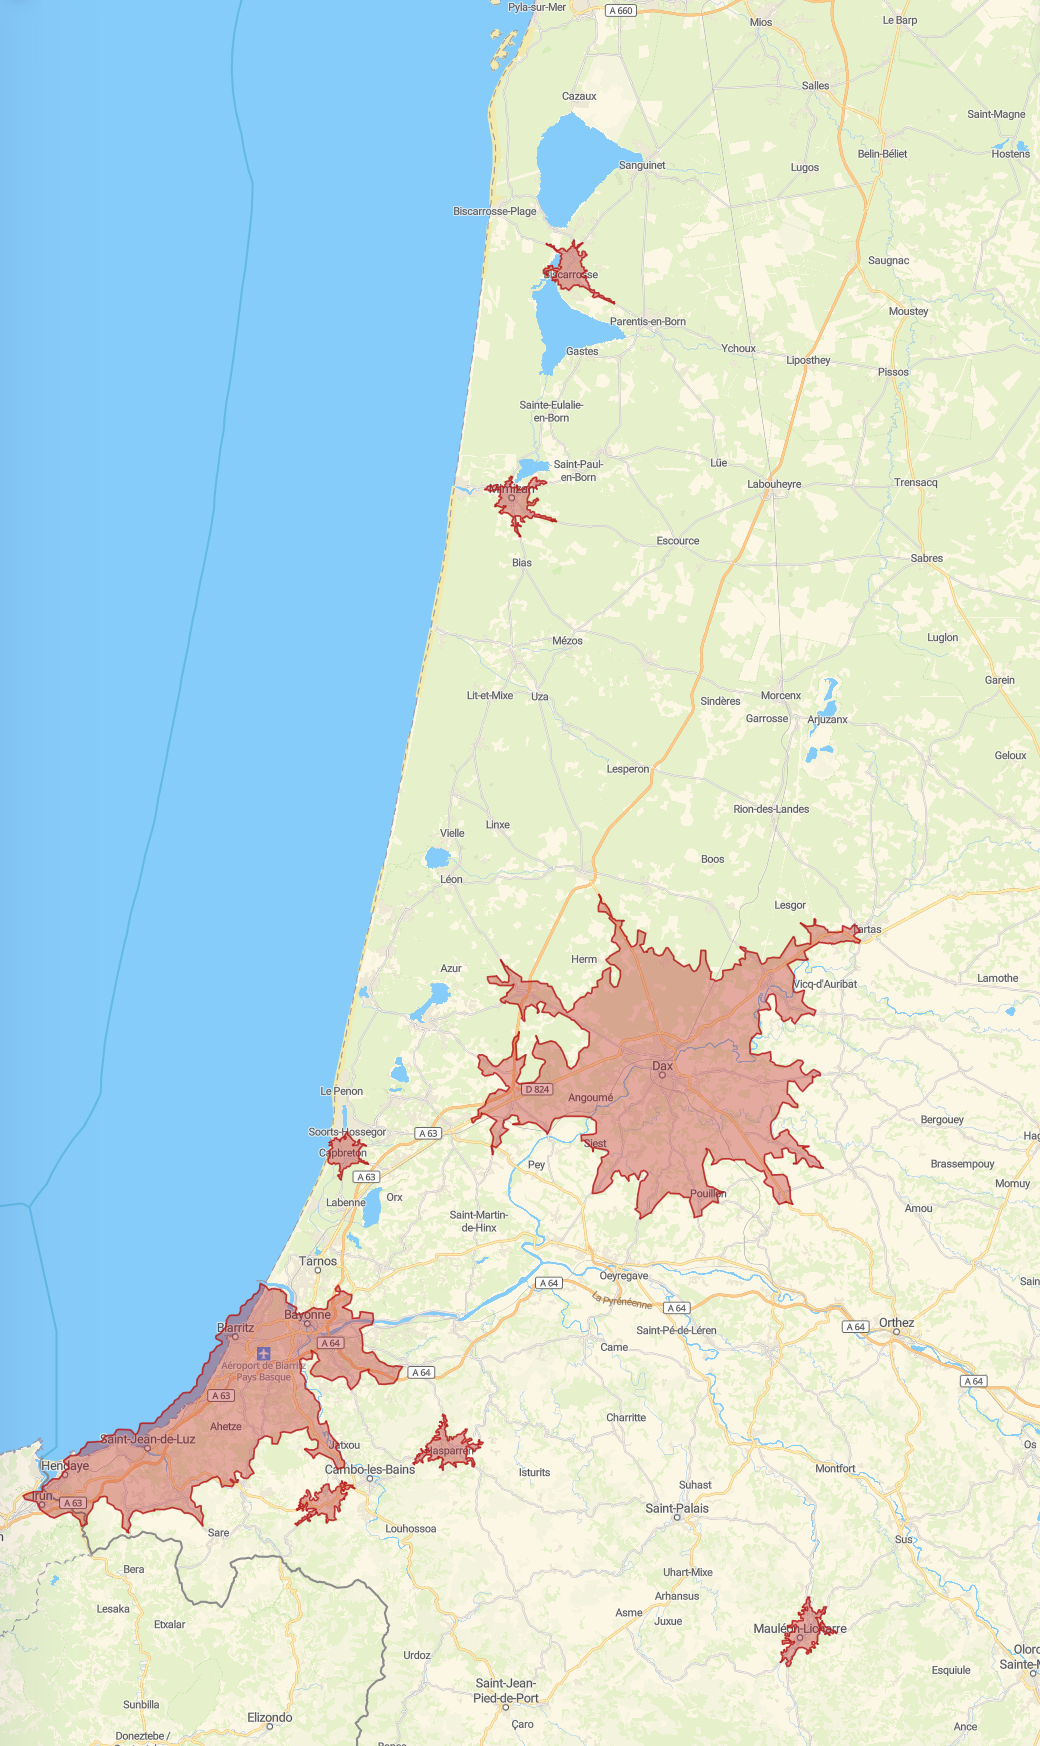
\includegraphics[width=\textwidth - \textwidth / 5]{zone_chalandise_aditu.png}
%     %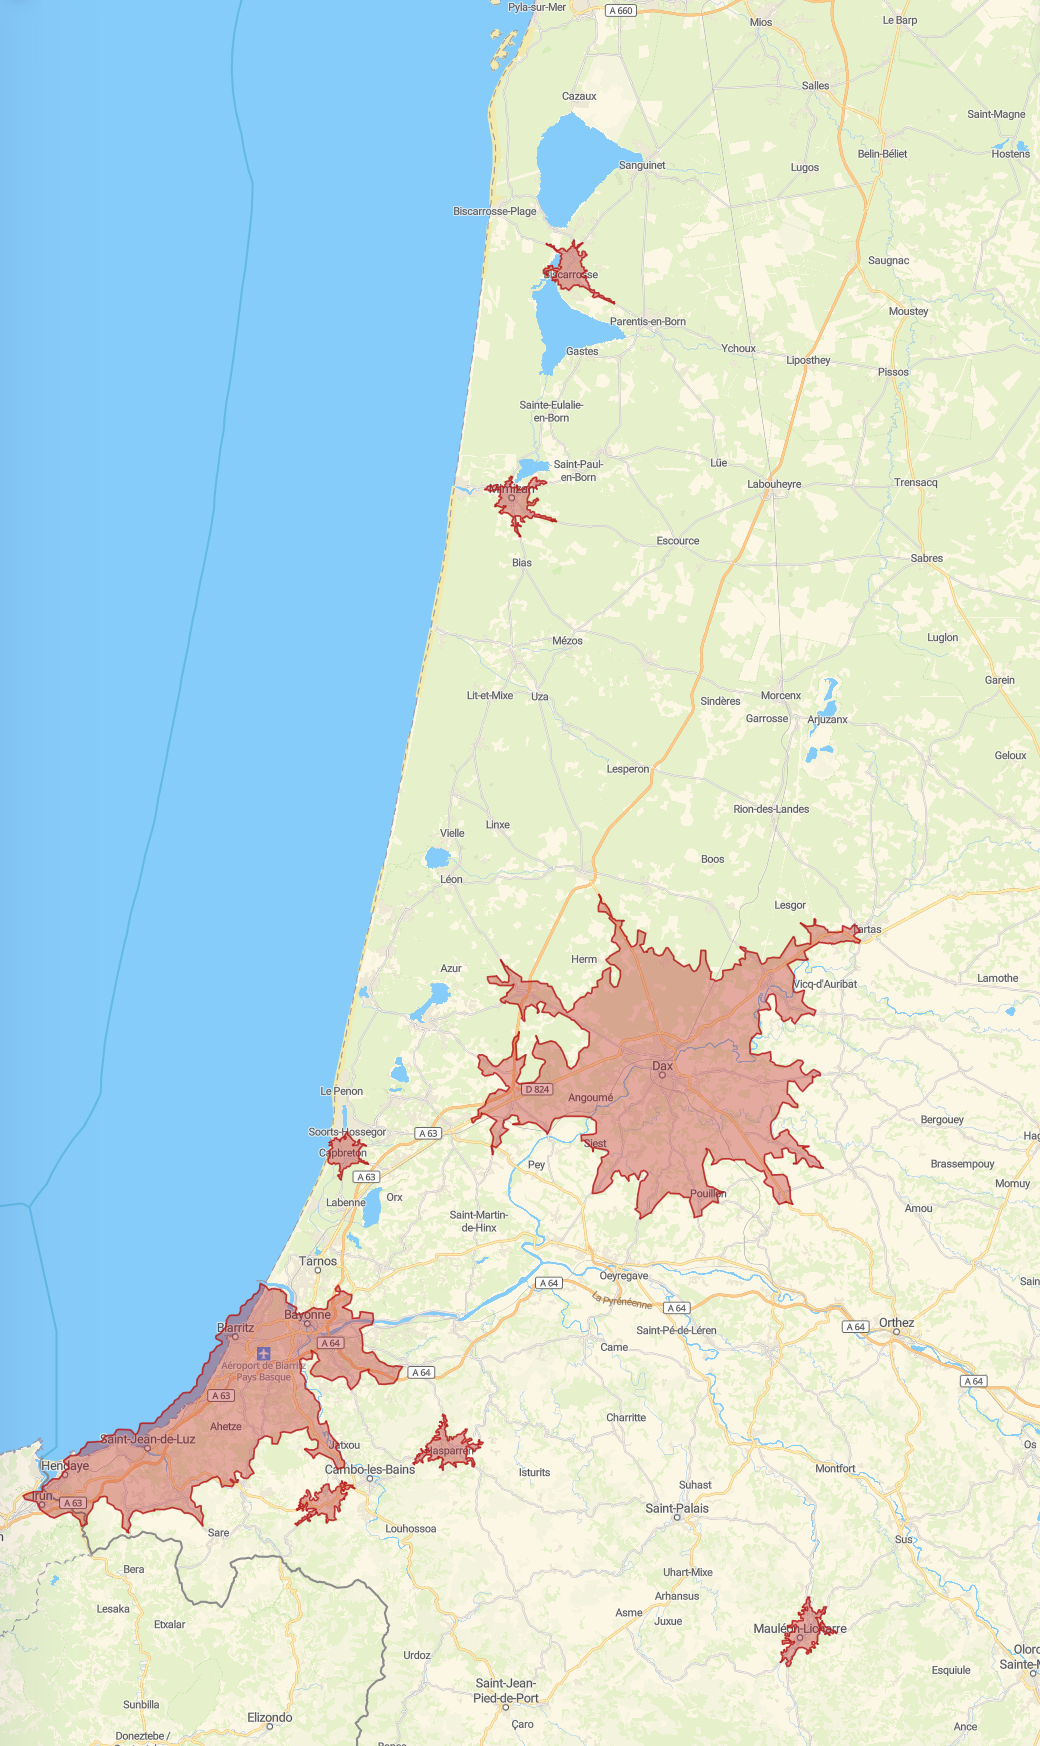
\includegraphics[scale=0.2]{zone_chalandise_aditu.png}
%     \figurename
%     \caption{Visualisation de la zone de chalandise d'ADITU, regroupée autour de ses datacenters à Bidart et à Dax}
%     \label{fig:zone_chalandise}
% \end{figure}

% \section{Cahier des charge Ticketing}

% % \begin{figure}[H]
% %     \centering
% %     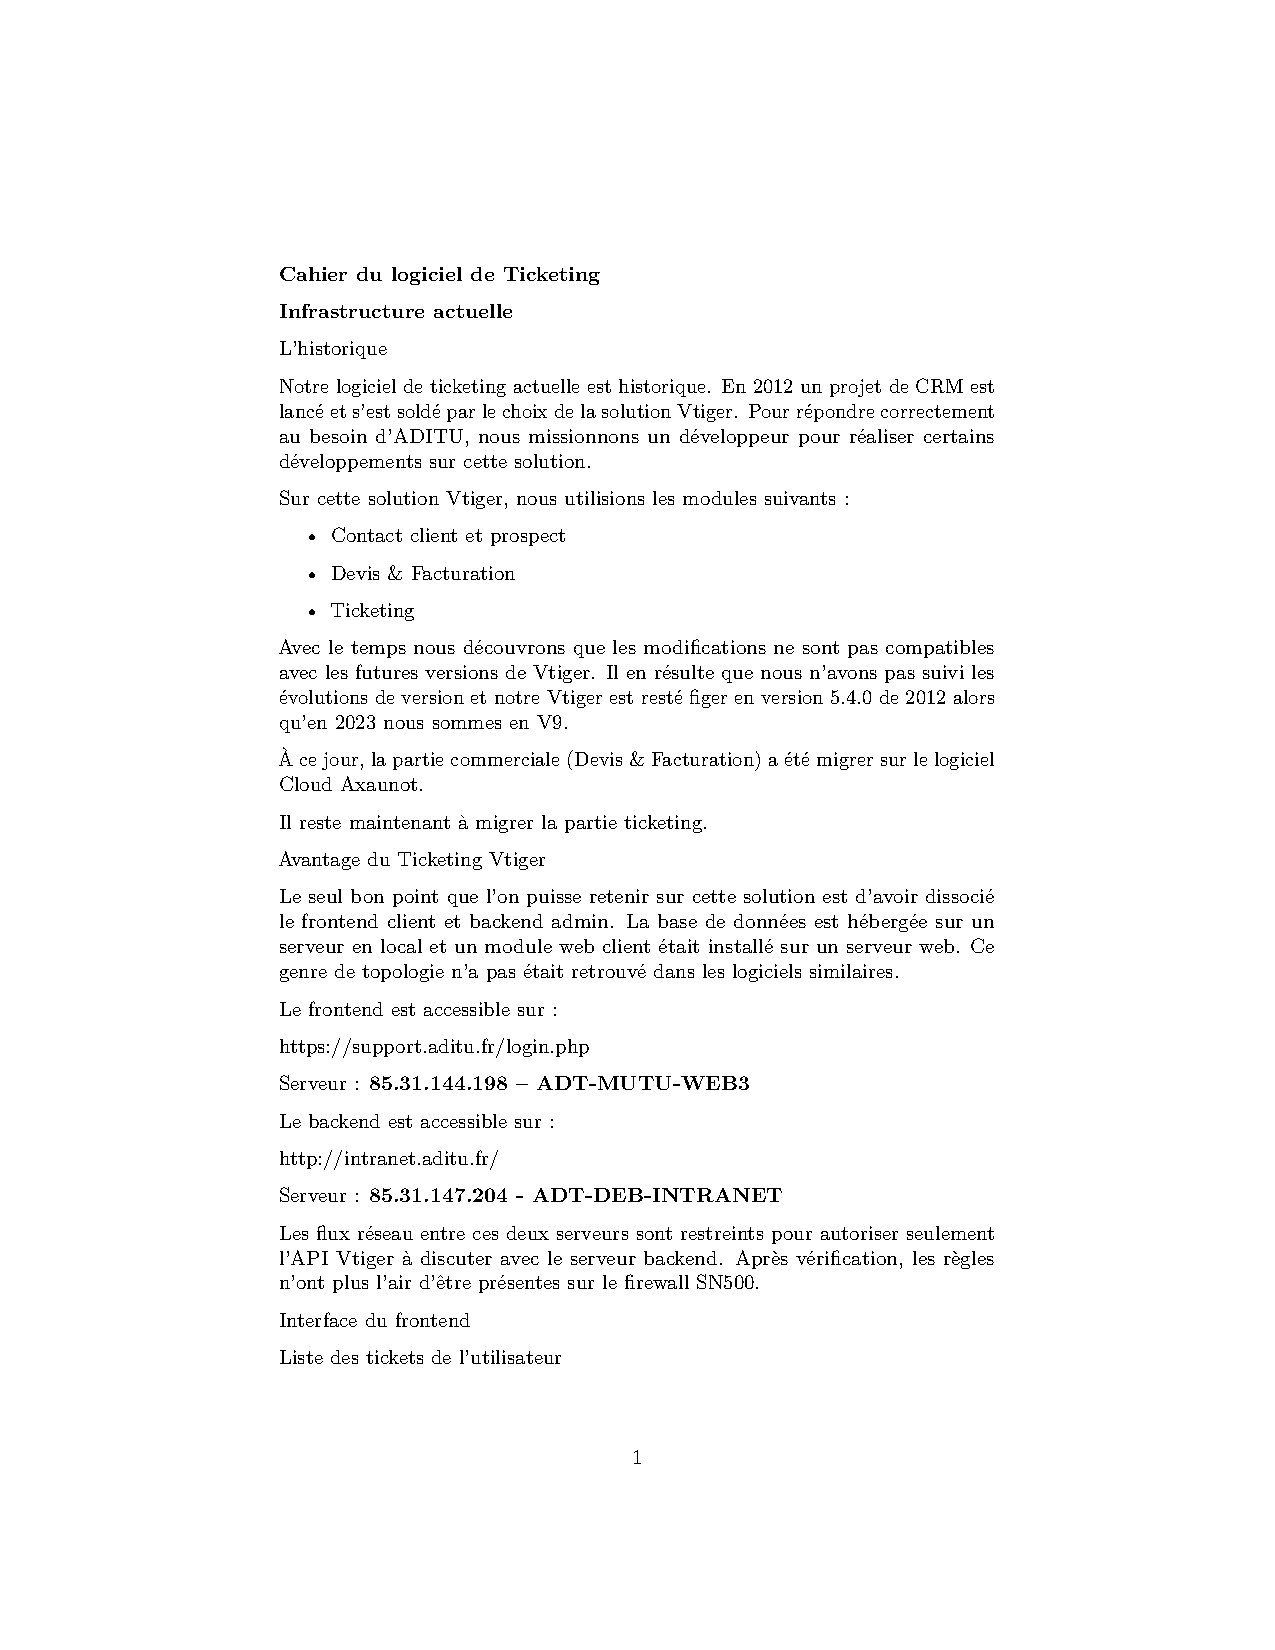
\includegraphics[width=\textwidth - \textwidth / 20]{CDC-Ticketing.pdf}
% %     \figurename
% %     \caption{Fiche de poste de notre alternance}
% %     \label{fig:poste}
% % \end{figure}

% \textbf{Cahier du logiciel de Ticketing}

% \textbf{Infrastructure actuelle}

% L'historique

% Notre logiciel de ticketing actuelle est historique. En 2012 un projet
% de CRM est lancé et s'est soldé par le choix de la solution Vtiger. Pour
% répondre correctement au besoin d'ADITU, nous missionnons un développeur
% pour réaliser certains développements sur cette solution.

% Sur cette solution Vtiger, nous utilisions les modules suivants~:

% \begin{itemize}
% \item
%   Contact client et prospect
% \item
%   Devis \& Facturation
% \item
%   Ticketing
% \end{itemize}

% Avec le temps nous découvrons que les modifications ne sont pas
% compatibles avec les futures versions de Vtiger. Il en résulte que nous
% n'avons pas suivi les évolutions de version et notre Vtiger est resté
% figer en version 5.4.0 de 2012 alors qu'en 2023 nous sommes en V9.

% À ce jour, la partie commerciale (Devis \& Facturation) a été migrer sur
% le logiciel Cloud Axaunot.

% Il reste maintenant à migrer la partie ticketing.

% Avantage du Ticketing Vtiger

% Le seul bon point que l'on puisse retenir sur cette solution est d'avoir
% dissocié le frontend client et backend admin. La base de données est
% hébergée sur un serveur en local et un module web client était installé
% sur un serveur web. Ce genre de topologie n'a pas était retrouvé dans
% les logiciels similaires.

% Le frontend est accessible sur~:

% \url{https://support.aditu.fr/login.php}

% Serveur~: \textbf{85.31.144.198 -- ADT-MUTU-WEB3}

% Le backend est accessible sur~:

% \url{http://intranet.aditu.fr/}

% Serveur~: \textbf{85.31.147.204 - ADT-DEB-INTRANET}

% Les flux réseau entre ces deux serveurs sont restreints pour autoriser
% seulement l'API Vtiger à discuter avec le serveur backend. Après
% vérification, les règles n'ont plus l'air d'être présentes sur le
% firewall SN500.

% Interface du frontend

% Liste des tickets de l'utilisateur

% 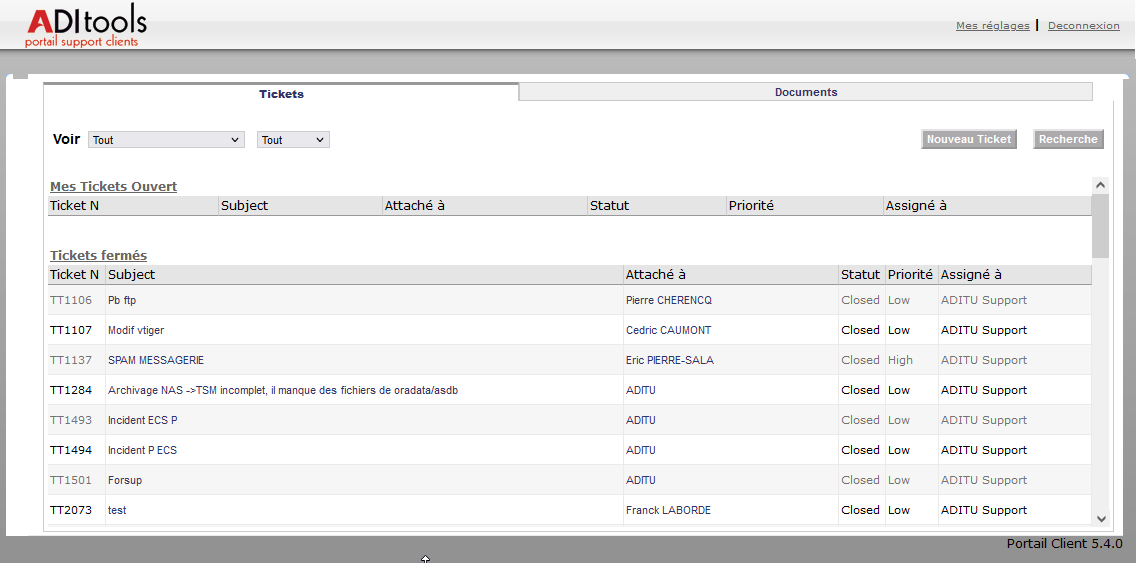
\includegraphics[width=6.3in,height=3.12222in]{image1.png}

% Création de tickets

% 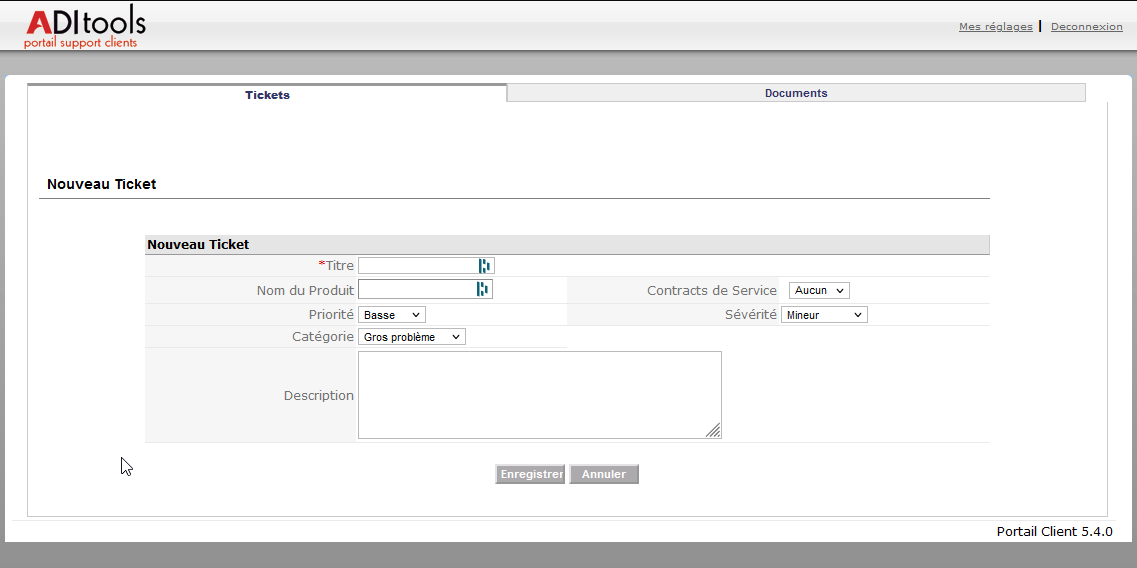
\includegraphics[width=6.3in,height=3.14722in]{image2.png}

% On peut constater que l'interface est plutôt minimaliste et
% vieillissante. Il manque certaines fonctions qui seront abordées plus
% bas.

% \textbf{Nouveau logiciel souhaité}

% Nous souhaitons migrer vers un nouveau logiciel de ticketing qui puisse
% intégrer les fonctionnalités ci-dessous~:

% Création d'incidents

% \begin{quote}
% La gestion des incidents permet de suivre et de résoudre les incidents
% signalés par les utilisateurs.
% \end{quote}

% Création de demandes de changement

% \begin{quote}
% Gestion des changements permet de planifier, suivre et gérer les
% modifications demandées par les utilisateurs.

% Exemple~: modification de ports sur le firewall, augmenter une boite aux
% lettres, etc.
% \end{quote}

% Création de tickets automatiquement

% \begin{quote}
% Cette fonctionnalité permet de planifier des interventions récurrentes
% sans les oublier. Exemple~: test de restauration
% \end{quote}

% Gestion des ressources

% \begin{quote}
% Pouvoir lié du matériel ou logiciel a un client et faire un suivi des
% modifications sur ce cette ressource.

% Exemple~: avoir le suivi des modifications comme celui qui est présent
% sur la page client du wiki.

% Intégrer du matériel lié à un fournisseur et gérer sa garantie. Exemple
% NAS ANANDA.

% Gérer les renouvellements~: des certificats

% Gérer les renouvellements~: des noms de domaines
% \end{quote}

% Inventaires

% \begin{quote}
% Lister l'ensemble des machines (connecteur OCS)
% \end{quote}

% Tableaux de bord et rapports

% Avoirs des stats et indicateurs sur ce qui nous prend le plus de temps
% dans le support.

% Ergonomique

% \begin{quote}
% Il faut que le logiciel soit intuitif et ergonomique. Que l'utilisateur
% ne soit pas rebuté par la complexité d'ouverture d'un ticket.
% \end{quote}

% Ouverture de ticket via email

% Fermeture de ticket automatique après un délai de non-réponse

% Personnalisation graphique

% \begin{quote}
% Nous souhaitons que l'application puisse se personnaliser aux couleurs
% de la société et d'y insérer le logo.
% \end{quote}

% Récupération des données ticketing vtiger

% \begin{quote}
% Seulement si cette récupération est facile. Ne pas perdre du temps sur
% cette récupération.
% \end{quote}

% Fonctions annexes

% Gestion des baies racks du datacenter


    % Pós Textuais
    % \nocite{*}
    % \include{pos-textuais/referencias}

\end{document}
